\documentclass[%
 reprint,
%superscriptaddress,
%groupedaddress,
%unsortedaddress,
%runinaddress,
%frontmatterverbose, 
%preprint,
%showpacs,preprintnumbers,
%nofootinbib,
%nobibnotes,
%bibnotes,
 amsmath,amssymb,
 aps,
%pra,
%prb,
%rmp,
%prstab,
%prstper,
%floatfix,
]{revtex4-1}

\usepackage{graphicx}% Include figure files
\usepackage{dcolumn}% Align table columns on decimal point
\usepackage{bm}% bold math
%\usepackage{hyperref}% add hypertext capabilities
%\usepackage[mathlines]{lineno}% Enable numbering of text and display math
%\linenumbers\relax % Commence numbering lines

%\usepackage[showframe,%Uncomment any one of the following lines to test 
%%scale=0.7, marginratio={1:1, 2:3}, ignoreall,% default settings
%%text={7in,10in},centering,
%%margin=1.5in,
%%total={6.5in,8.75in}, top=1.2in, left=0.9in, includefoot,
%%height=10in,a5paper,hmargin={3cm,0.8in},
%]{geometry}

\usepackage{cmap} % Поиск в PDF
\usepackage[T2A]{fontenc} % Кодировка
\usepackage[utf8]{inputenc} % Кодировка исходного текста
\usepackage[english, russian]{babel} % Локализация и переносы
\frenchspacing % Более тонкая настройка пробелов 
\usepackage{multirow}
\usepackage[warn]{mathtext}
\usepackage{amssymb}
\usepackage{ dsfont }
\usepackage{ textcomp }
\usepackage{ mathrsfs }

% Переопределение англоязычного начертания каппа, фи и эпсилон, 
% а также знаков сравнения
\renewcommand{\epsilon}{\ensuremath{\varepsilon}}
\renewcommand{\phi}{\ensuremath{\varphi}} 
\renewcommand{\kappa}{\ensuremath{\varkappa}}
\renewcommand{\le}{\ensuremath{\leslant}}
\renewcommand{\leq}{\ensuremath{\leqslant}}
\renewcommand{\ge}{\ensuremath{\geslant}}
\renewcommand{\geq}{\ensuremath{\geqslant}}
\renewcommand{\emptyset}{\ensuremath{\varnothing}}

\usepackage{textcomp} 
\usepackage{indentfirst} % Красная строка
\usepackage{amsmath} % Текст в формулах
\usepackage{graphicx} % Графика
\DeclareGraphicsExtensions{.pdf,.png,.jpg}
\usepackage{pgfplots}
\pgfplotsset{compat=1.13}

%\usepackage{times}

\begin{document}

\title{Интерференция лазерного излучения}
\thanks{4.5.2}

\author{Иван Едигарьев}
\affiliation{
 Московский Физико-Технический Институт\\
 Факультет Общей и Прикладной Физики, 526т\\
}
%\date{\today}

\begin{abstract}
Цель работы: исследовать зависимость видности интерференционной картины от угла $\beta$ между плоскостями поляризации интерферирующих волн при нулевой разности хода, зависимость видности интерференционной картины от разности хода интерферирующих пучков для угла $\beta = 0$. По результатам измерений следует оценить спектральные характеристики лазерного излучения: ширину спектра генерации и число генерируемых мод.

\end{abstract}

\pacs{Valid PACS appear here}% PACS, the Physics and Astronomy
                             % Classification Scheme.
%\keywords{Suggested keywords}%Use showkeys class option if keyword
                              %display desired
\maketitle

%\tableofcontent

\begin{enumerate}

    \item 
    Исследуем зависимость видности интерференционной картины от угла $\beta$ поворота первого поляроида при нулевой разности хода $(\nu_2 = 1)$: включим блок питания фотодиода и измерим величины $h_1, h_2, h_3, h_4$ на экране осциллографа. 
    
    \item
    Исследуем зависимость видности от разности хода между пучками. Для этого установим первый поляроид в положение, в котором интерференционная картина видна наиболее чётко $(\beta~=~0$\textdegree$, \nu_3 = 1)$. Снимем зависимость величин $h_1, h_2, h_3, h_4$ от координаты $x$ второго блока, начиная с минимального расстояния $(x = 12~cm)$.
    
    \item
    Рассчитаем коэффициент $\nu_3$. Построим графики $\nu_3(cos(\beta))$ и $\nu_3(cos(\beta)^2)$. 
    
    \begin{figure}[h]
    \center{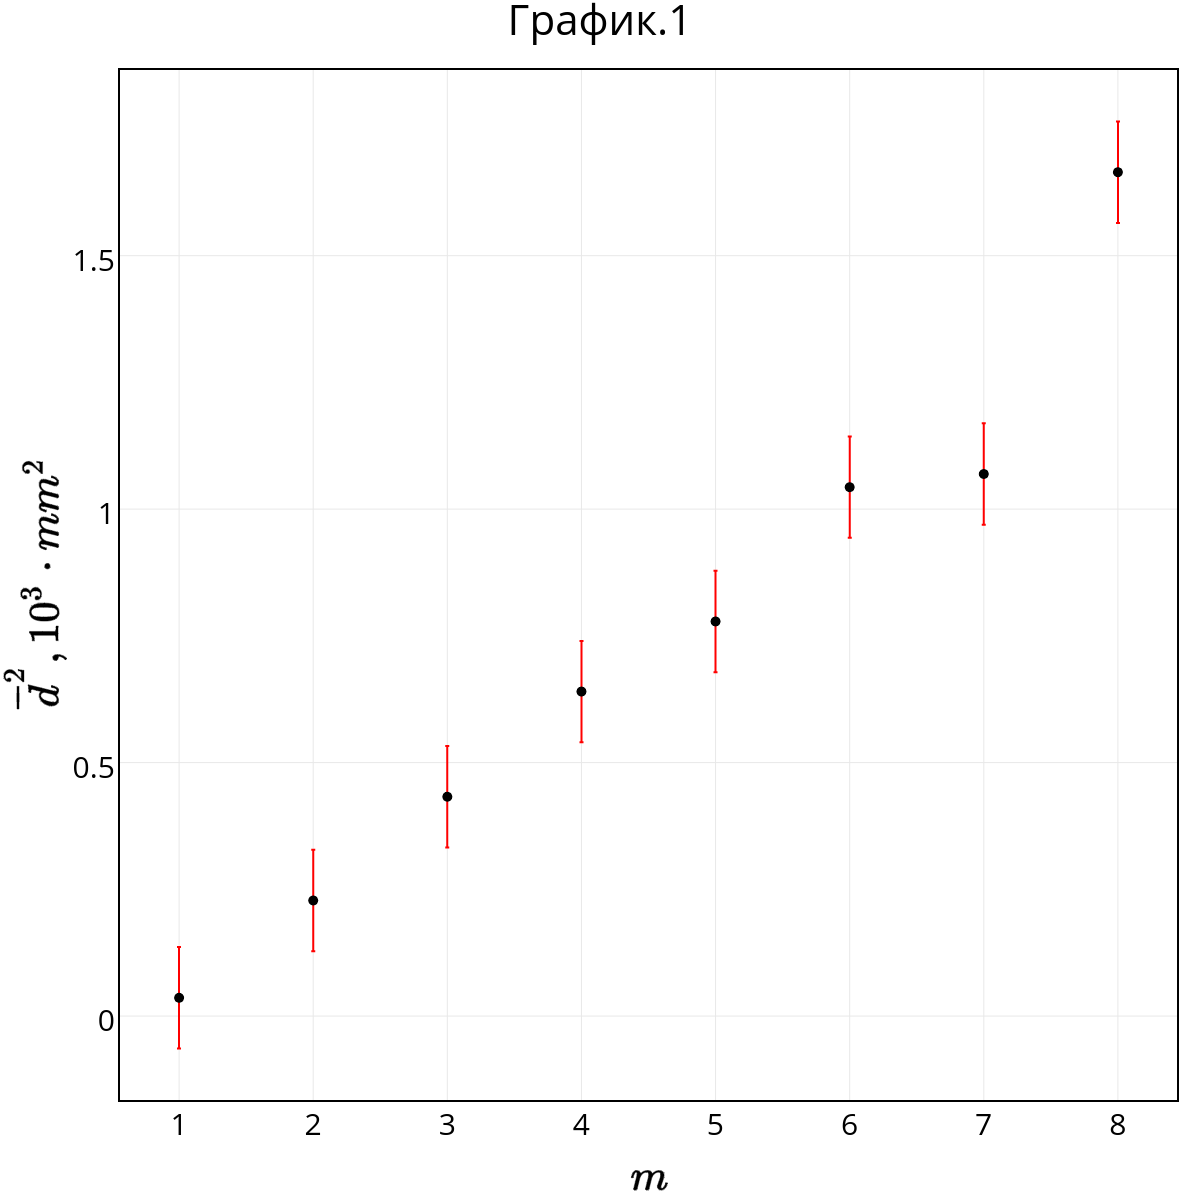
\includegraphics[scale=0.17]{my_plot1.png}}
    \end{figure}
    
    Легко видеть, что с точностью определяемой систематической ошибкой проведённых измерений теоретическая гипотеза о линейной зависимости показателя видности от $|cos(\beta)|$ выполняется.
    
    \begin{figure}[h]
    \center{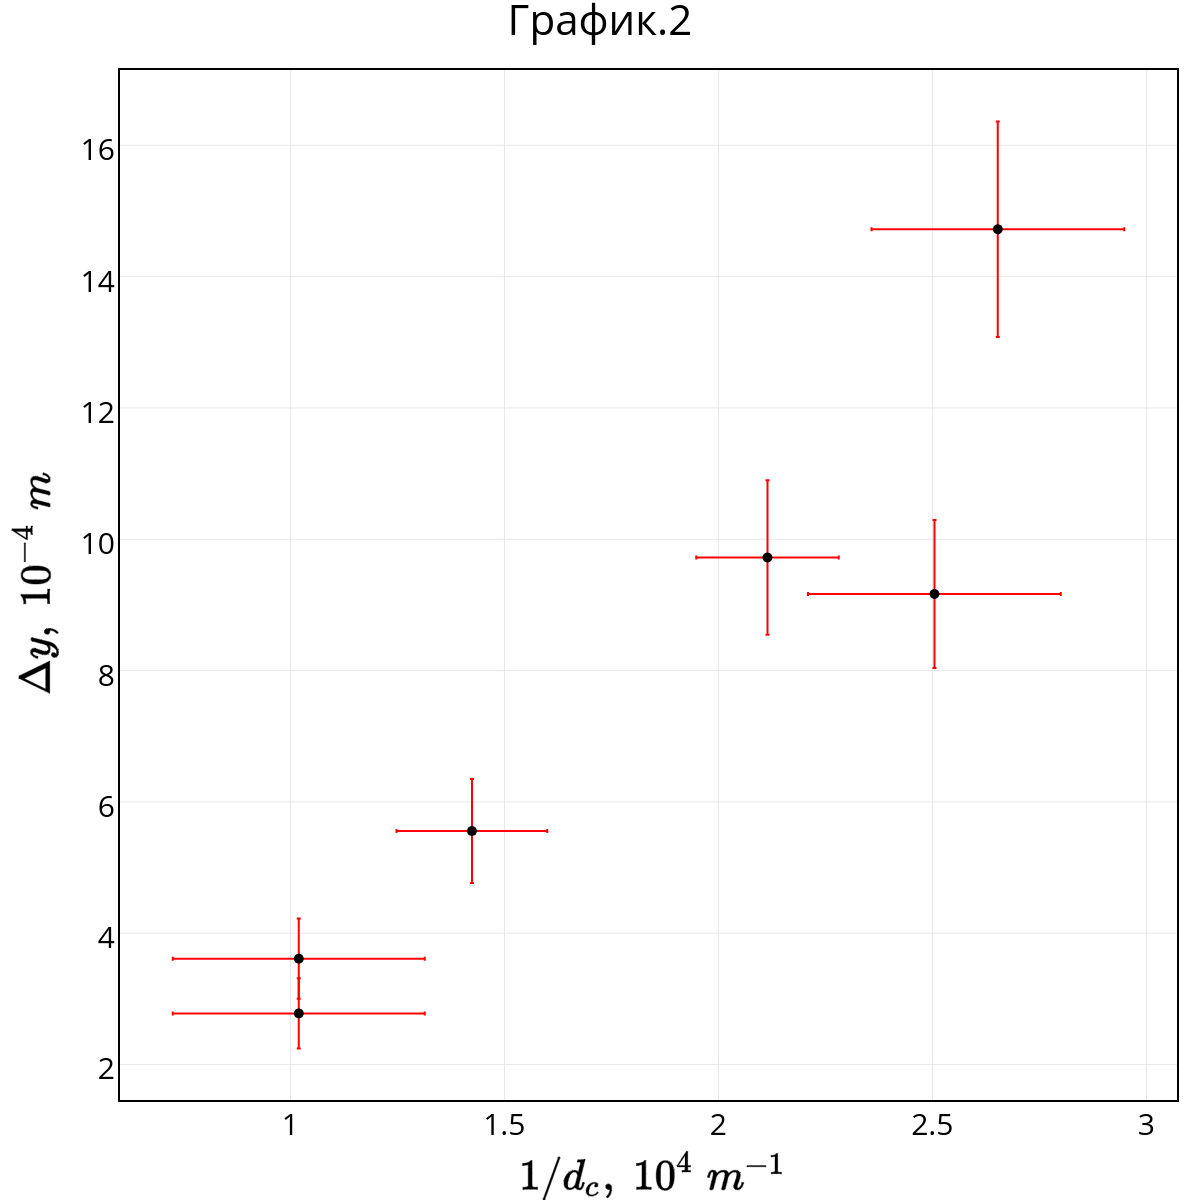
\includegraphics[scale=0.17]{my_plot2.png}}
    \end{figure}
    
    \item
    Рассчитаем коэффициент $\nu_2$. Построим график зависимости видности $\nu_2(x)$ от координаты второго блока. Определим по графику расстояния между максимумами, оценим расстояние $L$ между зеркалами оптического резонатора лазера и межмодовое расстояние $\Delta \nu_m$. 
    
    \begin{figure}[h]
    \center{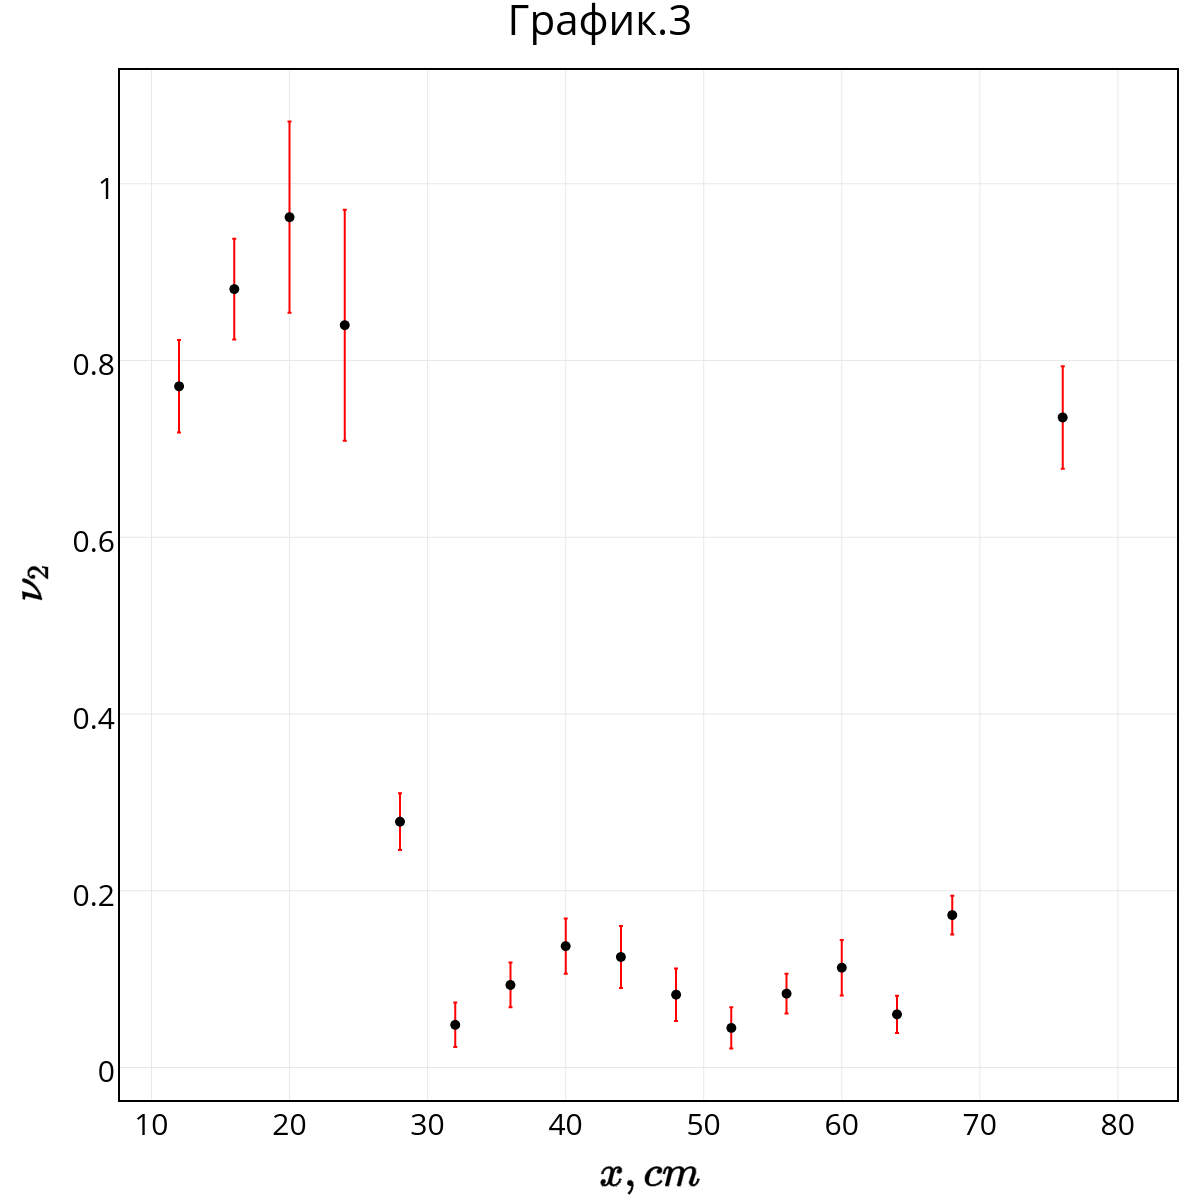
\includegraphics[scale=0.17]{my_plot3.png}}
    \end{figure}
    
    \begin{gather*}
        L = (30 \pm 5)~\text{cm}\\
        \Delta \nu_m = (5 \pm 1)~10^{8}~\text{s}^{-1}\\
    \end{gather*}

    \item
    Определим задержку $l_{1/2}$ (полуширину) на половине высоты главного максимума и рассчитаем диапазон частот $\Delta \nu_{\text{полн}}$, в котором происходит генерация продольных мод. Оценим число генерируемых лазером продольных мод.
    
    \begin{gather*}
        l_{1/2} = (10 \pm 2)~\text{cm}\\
        \Delta \nu_{\text{полн}} \approx \frac{0.6 c}{l_1
        {1/2}} = (1.8 \pm 0.4)~\text{s}^{-1}\\
        n \approx (5 \pm 1)\\
    \end{gather*}

    Стоит заметить, что все расчёты несут исключительно оценочный характер и верны только в границах обозначенных погрешностей. 
    
    
\end{enumerate}

\end{document}

